%%%%%%%%%%%%%%%%
%% Preambule  %%
%%%%%%%%%%%%%%%%

\documentclass[11pt]{article}

\usepackage{amsmath,amsfonts,amssymb}
\usepackage{upgreek}
\usepackage{enumerate}
\usepackage{multicol}
\usepackage{scrextend}

\usepackage[all]{xy}
\usepackage{tikz-qtree}
\usepackage[margin=2.5cm]{geometry}

\usepackage{fancyhdr}
\usepackage{lastpage}
\usepackage{tikz}

\setlength{\parindent}{0pt}

\pagestyle{fancy}

\lhead{\opdrachtNaam\ \opdrachtNummer}
\rhead{\naam(\studentNummer)}
\rfoot{Pagina\ \thepage\ van\ \pageref{LastPage}}
\lfoot{\datum}
\cfoot{}

\renewcommand\headrulewidth{0.4pt}
\renewcommand\footrulewidth{0.4pt}

\newcommand{\E}{\exists}
\newcommand{\A}{\forall}

\newcommand{\ccen}[2]{\llap{$#1$}${}\mathrel{\circ}{}$\rlap{$#2$}}

%%%%%%%%%%%%%%
%% Gegevens %%
%%%%%%%%%%%%%%

% Vul hier je gegevens in.

\newcommand{\naam}          {Stefan Schenk}
\newcommand{\studentNummer} {11881798}
\newcommand{\opdrachtNaam}  {Assignment}
\newcommand{\opdrachtNummer}{1}
\newcommand{\datum}         {02-11-17}

%%%%%%%%%%%%%%%%
%% Antwoorden %%
%%%%%%%%%%%%%%%%

\begin{document}


\section*{Opgave 2.7}
\textit{Bewijs de idempotentie, commutativiteit en associativiteit van
$ \cap $.}
\\

\textbf{Proof} idempotentie: $ A \cap A = A $

A random x is contained in $ A \cap A $ iff x in A and x in A.

$ \therefore $ x in A.

\textbf{Proof} commutativiteit: $ A \cap B = B \cap A $

A random x is in $ A \cap B $ iff x in A and x in B.

Then x in A and x in B. Thus also x in B and x in A.

$ \therefore $ x in $ B \cap A $.

\textbf{Proof} associativiteit: $ A \cap (B \cap C) = (A \cap B) \cap C $

A random x is contained in $ A \cap (B \cap C) $ iff x in A and x in
$ (B \cap C) $.

Recursively the same holds for x is contained in B and C.

Then x is in A, B and C, so x is in $ (A \cap B) $ and in C.

$ \therefore $ x in $ (A \cap B) \cap C $.


\section*{Opgave 2.17}
\textit{Laat zien dat uit de definitie van asymmetrie volgt dat elke asymmetrische relatie irreflexief is.}
\\

\textbf{Definition} assymmetric: Een relatie R $ \subseteq A^2 $ heet asymmetrisch wanneer voor geen enkel paar $ \langle a, b \rangle \in R $ geldt dat $ \langle b, a \rangle \in R $.
\\

A reflexive pair $ \langle a, a \rangle \in R $ can also be reversely written as: $ \langle a, a \rangle $. By assymmetry, this relation is not assymmetric.

$ \therefore $ in order for R to be irreflexive, it must be asymmetric.


\section*{Opgave 2.19}
\textit{Teken een plaatje van een relatie die noch transitief, noch intransitief is.}
\\

\begin{figure}[ht!]
\centering
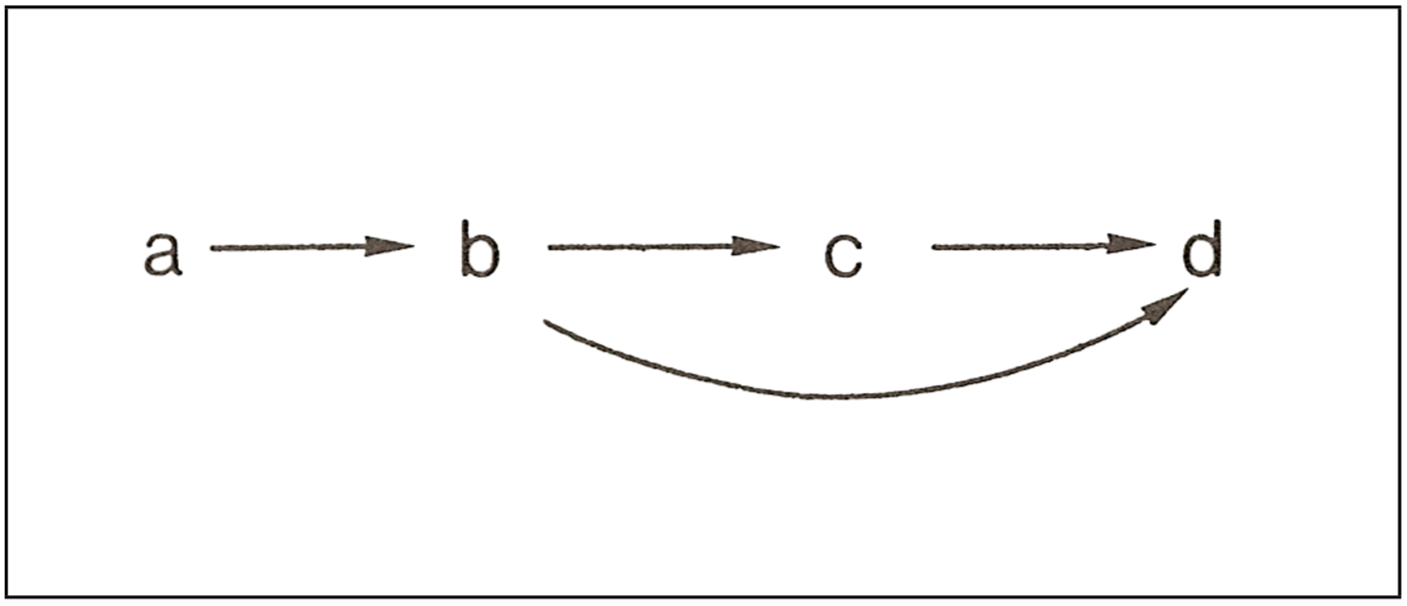
\includegraphics[width=90mm]{image1.png}
\caption{Not transitive, not intransitive \label{overflow}}
\end{figure}

\section*{Opgave 2.20}
\textit{1. Laat zien dat een asymmetrische relatie altijd anti-symmetrisch is.}
\\

An asymmetric relation has no pair $ \langle a, b \rangle $ that can be written as $ \langle b, a \rangle $, therefore there is no pair for which antisymmetry can be tested. Therefore it can be said that every asymmetric relation is also antisymmetrical.
\\

\textit{2. Laat zien dat het omgekeerde niet geldt. U kunt dit laten zien door een voorbeeld te geven van een anti-symmetrische relatie die niet asymmetrisch is.}
\\

Assuming there is an antisymmetrical pair, this pair can be written in reverse order, therefore the relation is not asymmetrical.


\section*{Opgave 2.23}
\textit{Laat zien dat elke strikte partiele orde bevat is in een partiele orde.}
\\

A partitial order in comparison with a strict partitial order, has extra pairs for reflexivity and antisymmetry. The strict partitial order, compared with a partitial order lacks these pairs because it is irreflexive instead of reflexive, and assymetric instead of antisymmetric. All the pairs that are made because a strict partitial order is transitive, are also contained in a partitial order, because it is also transitive.


\section*{Opgave 2.32}
\textit{N is de verzameling van natuurlijke getallen (de verzameling \{0,1,2,3,...\}, en $ f : N \rightarrow N $ is de functie ‘met 2 vermenigvuldigen’ (dat wil zeggen f(0) = 0, f(1) = 2, f(2) = 4, enzovoorts). Is f surjectief? Injectief? Bijectief?} \\

$ x \neq y $
\\
$ f(x) = 2x $
\\
$ f(y) = 2y $
\\
$ 2x \neq 2y $
\\

This implies that every x has one and only one result.
\\

By counterexample, $ f(x) = 2x + 1$ maps to values that are never reached by $ f(x) = 2x $. This implies that the function is injective because each input maps to each output exactly once or zero times. This also implies that the relation is not surjective, because there are outputs that are not reached.

Therefore the relation is deemed not bijective, because the relation is not surjective.

\section*{Opgave 3.23}
\textit{Hoeveel elementen telt een representant van de equivalentieklasse
$[\mathcal{P}(\{\emptyset\})]=_1  $ ?} \\

2

\section*{Verzamelingenleer 6}
\textit{Formaliseer onderstaande phrases in de taal van de verzamelingenleer.}

\begin{enumerate}
\item "Er zijn mensen die een kat verzorgen."
\\
$ \{b \in M, k \in K : \langle b, k \rangle \in V \} \neq \emptyset $
\\
Uitspraak
\item "Sommige katten hebben geen baasje."
\\
$ \{x \in \emptyset, k \in K : \langle x, k \rangle \in B \} \neq \emptyset $
\\
Uitspraak
\item "Sommige mensen verzorgen de kat die ze bezitten."
\\
$ \{m \in M, k \in K : \langle m, k \rangle \in (V \cap B) \} \neq \emptyset $
\\
Uitspraak
\end{enumerate}

\section*{Verzamelingenleer 7}
\textit{Geef geen opsomming, maar gebruik verzamelingentaal.}

\begin{enumerate}
\item De patienten van Michielsen..
\\
$ \{x : \langle x, m \rangle \in P \} $
\\
Verzameling
\item Alle patienten van Stevens zijn tevens patient van Teunissen.
\\
$ \{x : \langle x, s \rangle \} \subseteq \{x : \langle x, t \rangle \in P \} $
\\
Uitspraak
\item Roelofse en Stevens hebben geen patient gemeen.
\\
$ \{x : \langle x, r \rangle \in P \} \cap \{x : \langle x, s \rangle \in P \} = \emptyset $
\\
Uitspraak
\item De relatie binnen K x K van personen die Karelse als huisarts hebben.
\\
$ K^2 = \{ \langle a, b \rangle \mid \langle a, k \rangle \in P $
  and $ \langle b, k \rangle \in P \}$
\\
Relatie
\end{enumerate}

\end{document}
